\documentclass[superscriptaddress,reprint,amssymb, amsmath,aps, pre]{revtex4-1}
\usepackage[utf8]{inputenc}
\usepackage[T1]{fontenc}
\usepackage{amsmath}
\usepackage{amsfonts}
\usepackage{amssymb}
\usepackage{graphicx}
\usepackage{bm}
\usepackage{grffile} %Allows figure file names with periods
\usepackage{xr} %use for supplementary material
\usepackage{xcolor}
\usepackage{epsfig}
\usepackage{graphicx}
\usepackage{amssymb}
\usepackage{enumerate}
\usepackage{enumitem}
\usepackage{float}
%\usepackage{lipsum}
% \usepackage{mathtools}
% \usepackage{subcaption}
% \usepackage{relsize}
% \usepackage{listings}
% \usepackage{color}
\usepackage{hyperref}
% \usepackage{relsize}
% \usepackage{commath}
\usepackage{dirtytalk}
\usepackage{titlesec}
\usepackage{relsize}
\usepackage{amsmath}
\usepackage{breqn}

\newcommand{\C}{\mathbb{C}}
\newcommand{\I}{\mathbb{I}}
\newcommand{\R}{\mathbb{R}}
\newcommand{\N}{\mathbb{N}}
\newcommand{\K}{\mathbb{K}}

\newcommand{\rd}{\textrm{d}}

\newcommand{\bc}{\textbf{c}}
\newcommand{\bbf}{\textbf{f}}
\newcommand{\bg}{\textbf{g}}
\newcommand{\bu}{\textbf{u}}
\newcommand{\bv}{\textbf{v}}
\newcommand{\bw}{\textbf{w}}
\newcommand{\bx}{\textbf{x}}
\newcommand{\by}{\textbf{y}}

\externaldocument[supp-]{CC_OA_comparison_supplementary}
\newcommand{\diag}[1]{\textrm{diag}\left(#1\right)}
\newcommand{\dbyd}[1]{\frac{\rd}{\rd#1}}
\newcommand{\re}[1]{\textrm{Re}\left(#1\right)}
\newcommand{\imag}[1]{\textrm{Im}\left(#1\right)}
\newcommand{\trace}[1]{\textrm{tr}\left(#1\right)}
\newcommand{\deriv}[2]{\dfrac{ d #1}{ d #2}}
\newcommand{\fn}[1]{f_{ #1}}

\renewcommand{\labelenumii}{\theenumii}
\renewcommand{\theenumii}{\theenumi.\arabic{enumii}.}
\newcommand\numberthis{\addtocounter{equation}{1}\tag{\theequation}}
\graphicspath{{figures/}}

\titlespacing\section{0pt}{12pt plus 4pt minus 2pt}{0pt plus 2pt minus 2pt}
\titlespacing\subsection{0pt}{12pt plus 4pt minus 2pt}{0pt plus 2pt minus 2pt}
\titlespacing\subsubsection{0pt}{12pt plus 4pt minus 2pt}{0pt plus 2pt minus 2pt}
% \titlespacing{\section}{0pt}{\parskip}{-\parskip}
% \titlespacing{\subsection}{0pt}{\parskip}{-\parskip}
% \titlespacing{\subsubsection}{0pt}{\parskip}{-\parskip}
\newcommand{\squeezeup}{\vspace{-3mm}}
%\DeclarePairedDelimiter{\ceil}{\lceil}{\rceil} %%for ceil


%%% first author
% \author{Ankith Anil Das
%     \affiliation{
%     470485327\\
% 	Faculty of Science, Mathematics\\
% 	The University of Sydney\\
%     Email: aani9804@uni.sydney.edu.au
%     }
% }
%\title{Model reduction for the collective dynamics of globally coupled oscillators}


\begin{document}
\title{An Extension of the Swarmalator Model}
\author{Ankith Anil Das}
\begin{abstract}
{
    \it Synchronization occurs at many natural and technological systems. Such an emergent properties is observed in cardiac pacemaker cells, Japanese tree frogs, colloidal suspensions of magnetic particles, and other biological and technological systems in which synchronization interact. We consider a system where phase dynamics and spacial dynamics are coupled. A detailed analysis of such a system was proposed by Kevin P. O'Keeffe in the paper \say{Oscillators the sync and swarm}. We studied an extension of the Swarmalator model proposed in the paper. Understanding the dynamics of this model could possibly give insight to the generalized model where the phase coupling function could be a fourier series.
}
\end{abstract}

\maketitle
%
%%%%%%%%%%%%%%%%%%%%%%%%%%%%%%%%%%%%%%%%%%%%%%%%%%%%%%%%%%%%%%%%%%%%%%

% %%%%%%%%%%%%%%%%%%%%%%%%%%%%%%%%%%%%%%%%%%%%%%%%%%%%%%%%%%%%%%%%%%%%%%
% \begin{nomenclature}
% \entry{A}{You may include nomenclature here.}
% \entry{$\alpha$}{There are two arguments for each entry of the nomemclature environment, the symbol and the definition.}
% \end{nomenclature}

% The primary text heading is  boldface and flushed left with the left margin.  The spacing between the  text and the heading is two line spaces.

% %%%%%%%%%%%%%%%%%%%%%%%%%%%%%%%%%%%%%%%%%%%%%%%%%%%%%%%%%%%%%%%%%%%%%%

\section{Introduction}
{
    Synchronization in oscillations occurs in many natural systems, including the activity of the brain\cite{Sheeba2008}, and synchronous firefly flashing\cite{Mirollo1990Synchronization}, as well as many engineering applications, such as power grids\cite{powerGrid}, and Josephson junction arrays\cite{Watanabe1994}. Kuramoto model \cite{kuramoto} was one of the first major analysis in synchronization of coupled oscillators. Kuramoto's discovery of critical coupling strength, above which causes spontaneous synchronization was a breakthrough in the dynamics of coupled oscillators. This model has been generalized to other large systems of biological oscillators, such as chorusing frogs\cite{Aihara2008}, firing neurons\cite{SpikingNeurons}, and even human concert audiences clapping in unison\cite{Clapping}. 

    One area which has come under recent light is the collective study of swarming and synchronization. Both synchronization and swarming involve large,self organizing groups which interact according to some set of simple rules. Studies involving swarming of animals focus on spacial dynamics, while ignoring internal state. On the other hand, studies involving synchronization focus on phase dynamics and not their motion. A combined model was proposed by O’Keeffe et al. \cite{swarm}, which looked into the collective dynamics of phase and position of oscillators. He called such oscillators ``swarmalators'' to highlight their dual nature. In this mini report, we will be looking into an extended model which has a more general phase coupling function. Our motivation for such an extension was to understand the behavioral changes of system, whose results could help us generalize the phase coupling function to a fourier sin series. 
}

\noindent
\section{The Model}
{
    We consider swarmalators free to move in the plane. The governing equations are \cite{swarm} 
    \begin{gather}
        \dot{\mathbf{x}}_{i}=\mathbf{v}_{i}+\frac{1}{N} \sum_{j=1}^{N}\left[\mathbf{I}_{\mathrm{att}}\left(\mathbf{x}_{j}-\mathbf{x}_{i}\right) F\left(\theta_{j}   -\theta_{i}\right)-\mathbf{I}_{\mathrm{rep}}\left(\mathbf{x}_{j}-\mathbf{x}_{i}    \right)\right] \\
        \dot{\theta}_{i}=\omega_{i}+\frac{K}{N} \sum_{j=1}^{N} H_{\mathrm{att}}\left(\theta_{j}-\theta_{i}\right) G\left(\mathbf{x}_{j}-\mathbf{x}_{i}\right)
    \end{gather}
    for \(i = 1,\ldots,N\), where \(N\) is the number of swarmalators, $\mathbf{x}_{i} $ is the position of the \(i\)-th swarmalator, and $\theta_i,\omega_i,$ and $\mathbf{v}_i$ are it's phase, natural frequency and background velocity. The functions $\mathbf{I}_  {att}$ and $\mathbf{I}_{rep}$ represent spatial attraction and repulsion between the swarmalators where as phase interaction is governed by $\mathbf{H}_{att}$. We considered the following model:
    \begin{gather} 
        \dot{\mathbf{x}}_{i}=\mathbf{v}_{i}+\frac{1}{N}\left[\sum_{j \neq i}^{N} \frac  {\mathbf{x}_{j}-\mathbf{x}_{i}}{\left|\mathbf{x}_{j}-\mathbf{x}_{i}\right|}\left  (1+J \cos \left(\theta_{j}-\theta_{i}\right)\right)-\frac{\mathbf{x}_{j}-\mathbf{x}_{i}}{\left|\mathbf{x}_{j}-\mathbf{x}_{i}\right|^{2}}\right] \label{eq:space} \\
        \dot{\theta}_{i}=\omega_{i}+\frac{K}{N} \sum_{j \neq i}^{N} \frac{\gamma_1 \sin\left(\theta_{j}-\theta_{i}\right) + \gamma_2 \sin \left(2 \left(\theta_j -\theta_i\right)\right) }{\left|\mathbf{x}_{j}-\mathbf{x}_{i}\right|} \label{eq:phase}
    \end{gather}
    %% State the differences of our model to the original swarmalator model 
    We considered identical swarmalators so that $\omega_i = \omega$ and $\mathbf{v}_i = \mathbf{v}$. Using this assumption, using a suitable choice of reference frame we  can set $\omega = 0$, and $\mathbf{v} = \mathbf{0}$. The system has four parameters $\left(J,K,\gamma_1,\gamma_2\right )$.

    The parameter \(J\) measures the extend to which phase similarity enhances spatial attraction. For $J>0$, swarmalators prefer to be near other swarmalators with  similar phase. When $J<0$, the opposite behavior is observed: swarmalators attract those with opposite phase. When $J=0$, they show no phase based spatial behavior,i.e, their spatial attraction is independent of phase. To maintain $\mathbf{I}_{att}> 0$, we constrain $J$ to $-1 \leq J \leq 1$. The parameter $K$ is the phase coupling strength which scales $\gamma_1$, and $\gamma_2$. The relative  strengths of $\gamma_1$ and $\gamma_2$ determine the stability of one or two clusters. 
    
    Before stating the dynamics of the system, we pause to state the features of this model. This model's purpose is to study the interplay between swarming and synchronization. Our model accounts for aggregation, but not alignment. There are no alignment terms.  We chose to neglect orientation because it adds another layer of complexity; it makes each swarmalator have four state variables. For rest of the report we will refer to our model as `Dual phase coupled model' because of the presence of double angle $\sin$ function in Eq.\ref{eq:phase}. In a similar fashion, the original model proposed by P. O'Keeffe will be referred as `Single phase coupled model'.\noindent
}
\section{Optimization of the ode solver}
{
    The simulations were run using MATLAB's ODE integrator `ode45'. Absolute and Relative tolerance for the integrator was set to $10^{-6}$. Before large computations were performed, optimisation of the existing code was necessary. As this project involves computations of large matrices using ode45, optimising the code for speed was essential for any extensive calculation. The initial code was profiled using MATLAB's performance profiler, and bottlenecks were identified. Calculating the pairwise inverse distance was the most computationally expensive part in the ode function. The original code took 70 seconds for a simulation with $N = 100$ and $T = 10$-time units. This speed was too slow for any extended time simulations. After removing unwanted function calls, changing the algorithm, and using functions which supports vectorization, the new code took 0.509 sec for the same task. The performance was good enough for an interactive user simulation where the user can change the parameters of the system and can see the results almost instantly.
}

\section{Cluster formation and stability}
{
    %One of the core objectives of this project was to understand the cluster formation and its stability.
    The dynamics of dual phase coupled model had some striking differences with the original single phase model. The system not only settled in all the five states which were discussed in detail by Kevin P. O'Keeffe in single phase model, but also showed many additional stable and metastable states. Understanding the behavior of the modified phase coupling term and how it affects the formation of states could give us deep insights about the generalization of the model.
    % Maybe modify this %
    The additional cluster states made by the model can be broadly classified as follows 
    \begin{enumerate}[label = (\alph*)]
        \item Static two cluster state
        \item Static bimodal single cluster state.
        \item Two cluster state with rogues 
        \item Active three-four cluster state
        \item Active single cluster state
    \end{enumerate}
    % add figures for the model%
    \noindent
    To understand system behavior under the change of \(\gamma_1\), and \(\gamma_2\), we chose \(J = 0.8\) and \(K = -0.5\) which represent Active phase wave in single phase coupled model. This set of state variables were chosen because it showed the most active spacial behavior in single phase coupled model and the dynamics of the system would be more depended on the values of \(\gamma_1\) and \(\gamma_2\). Unless otherwise stated, the simulations are run with \(J = 0.8\) and \(K = -0.5\). Also, all the simulations were run with random initial position in a 1x1 box and phases from \([-\pi, \pi]\), both uniformly and random. To maintain consistency, the same random seed was used for all simulations.
    \begin{figure}
        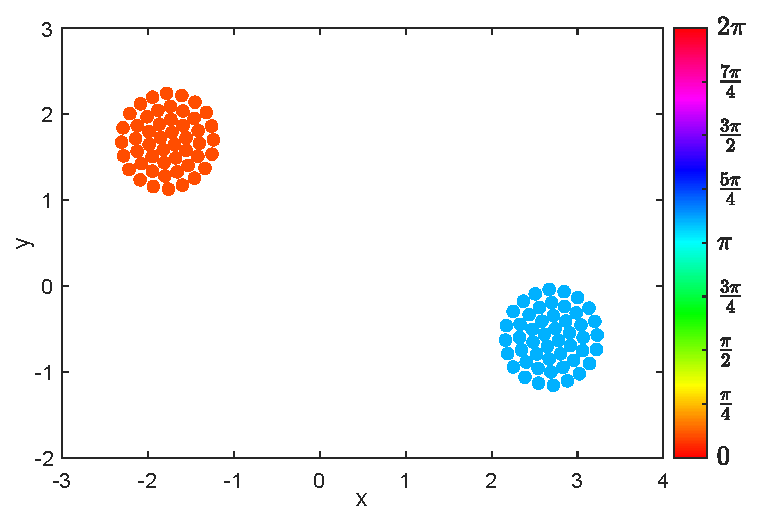
\includegraphics[width = \linewidth]{TwoCluster.eps}
        \caption{Static two Cluster State. This state was achieved for \(N = 100\), \(\gamma_1 = 2/3\), and \(\gamma_2 = -0.5\). The simulation was run for \(T = 100\) time steps with variable step-size (ode45) for the system to settle down.}
        %\vspace{-12mm}
        \label{fig:static2}
    \end{figure}
    \begin{figure}
        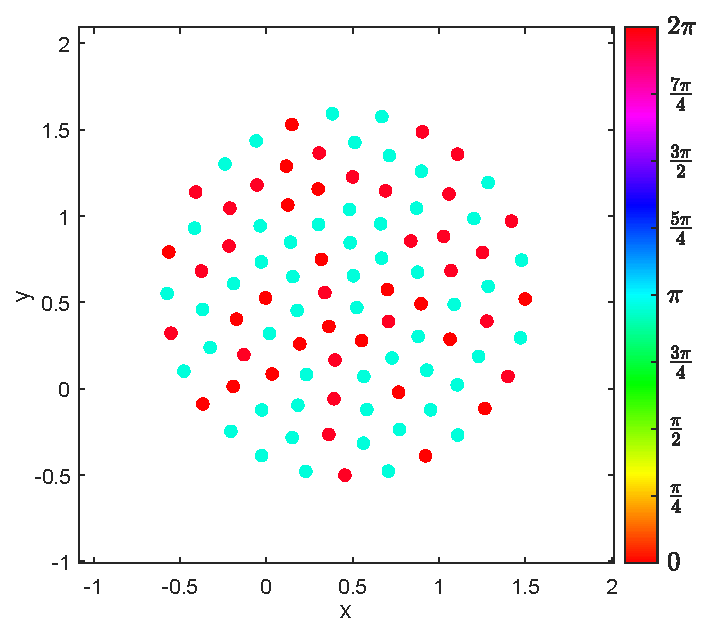
\includegraphics[width = \linewidth]{staticSingleClusterState.eps}
        \caption{Static bimodal single cluster state. This state was achieved for \(N = 100, K = -0.5,J = -0.8,\gamma_1 = 2/3,\gamma_2 = -0.1\) after \(T = 300\) time steps.}
        \label{fig:staticSingleClusterState}
    \end{figure}
    \begin{figure}
        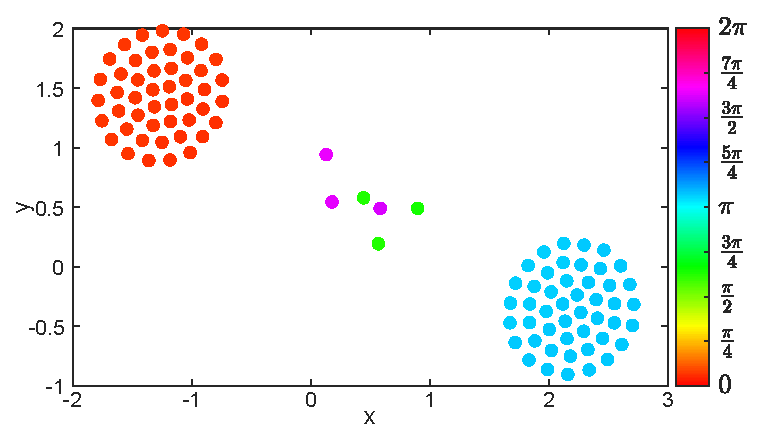
\includegraphics[width = \linewidth]{twoClustersWithR100.eps}
        \caption{Two Clusters with Rogues. This state was reach under a random run with \(\gamma_1 = 2/3,\gamma_2 = -1/3\) after \(T = 200 \) time steps.}
        \label{fig:twoClustersWithRogues}
    \end{figure}
    \begin{figure}
        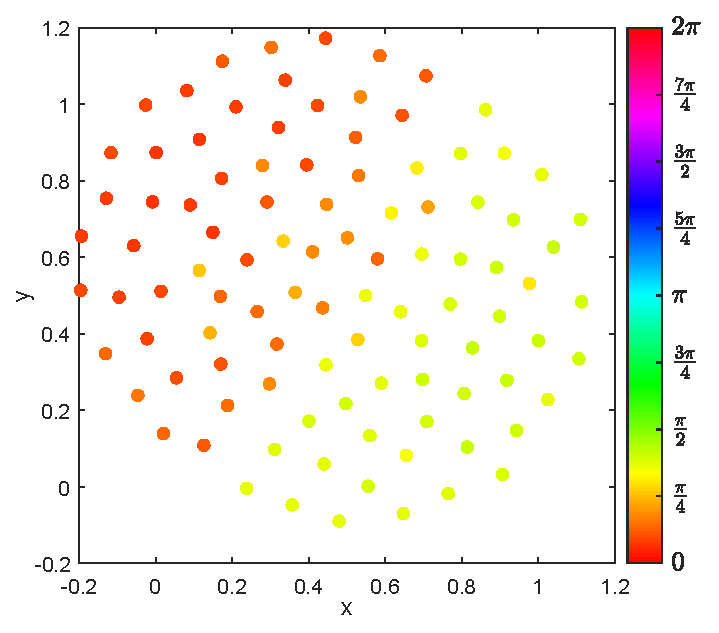
\includegraphics[width = \linewidth]{ActiveSingle.eps}
        \caption{Active Single cluster state.This state was achieved for \(N = 100\), \(\gamma_1 = -1\), and \(\gamma_2 = +0.72\). It is a non-stationary state where swarmalators on the boundary of the two phase clusters jump from one side of the cluster to other.}
        \label{fig:ActiveSingle}
    \end{figure}
    \begin{figure}
        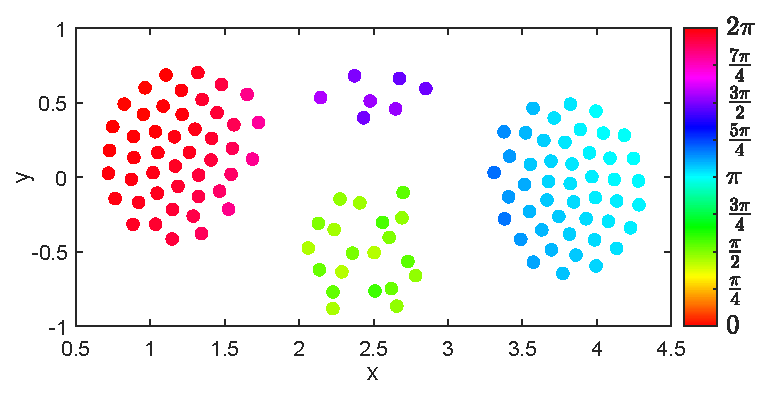
\includegraphics[width = \linewidth]{Active4Clust.eps}
        \caption{Active 4 cluster state. This special state was achieved by manually adding 20 swarmalators of phase \(\pi/2\) in the middle of two clusters with phase \(0\) and \(\pi\). The figure shows the state after \(T = 300\) time steps}
        \label{fig:Active4Clust}
    \end{figure}
    %% Phase distribution in 2 cluster state. 
    % Show a graph which shows phase with time and how it settles down.
    % Explain why such settling is expected
    % Discuss about the values of K J gamma1 and gamma2 values chosen for the sims 
    % Point out that a detailed explanation for the chosen gamma1 and gamma2 values will be discussed in the later section. 
    % Make a code to find the jacobian matrix and look at the stability of the system
    \section{Static Two cluster state}
    {
        Static two cluster case is a very common equilibrium state seen for various values of \((J,K,\gamma_1,\gamma_2)\), illustrated in  Fig.\ref{fig:static2}. Since \(J > 0\), `like attracts like': swarmalators want to settle near other swarmalators with similar phase. Looking at phase dynamics equation (Eq.\ref{eq:phase}) \(\dot{\theta}_{i} = 0\) when \(\theta_i = C, C + \pi \), where \(C\) is any constant. Due to the presence of a new stable phase, the system can form two clusters with \(\pi\) phase difference. Now for the given value of \(K\) which is less than 0, \(\gamma_1 > 0\) (Negative coupling) implies the system does not prefer single cluster state, and \(\gamma_2 < 0\) (positive coupling) means the system prefers to stabilize in two cluster state. Furthermore, \(|\gamma_2| > |\gamma_1|\) shows that the second coupling term in Eq.\ref*{eq:phase} is more dominant in stabilizing the system. Fig.\ref{fig:phasevsTime} shows how the phase settles with time. Here, the phase effectively stabilizes to two values after taking mod \(2\pi\). The average cluster phase difference is approximately \(\pi\) with an absolute error \(\epsilon \approx 2.6074 \times 10^{-9}\). Our statement about two cluster phase difference therefore agrees with the simulations. 

        \begin{figure}
            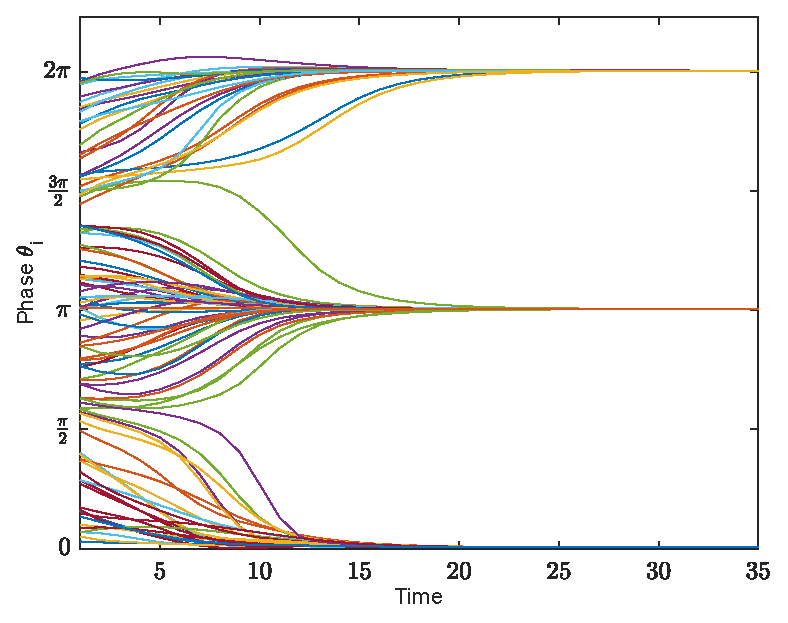
\includegraphics[width = \linewidth]{phasevstimeN_100.eps}
            \caption{Phase of the Swarmalator vs Time. }
            \label{fig:phasevsTime}
        \end{figure}
    }
    
    \subsection{Inter-cluster distance for Static two cluster state}
    {
        We can analytically solve the inter-cluster distance for static two cluster state by making an assumption.
        Let,
        \begin{align} %% Fix this stupid sum SIghISHFISHFOA
            \mathbf{C}_0 = \frac{1}{N_0} \sum_{i \in S_0 } \mathbf{x}_i &&\text{and}&& \mathbf{C}_\pi = \frac{1}{N_\pi} \sum_{i \in S_\pi } \mathbf{x}_i ,
        \end{align}
        where \(\mathbf{C}_0\) and \(\mathbf{C}_\pi\) are the centroids of the clusters with average phase approximately equal to \(0\) and \(\pi\) respectively , and \(S_0\) and \(S_\pi\) are the respective clusters. Differentiating \(\mathbf{C}_0\) w.r.t time gives 
        \begin{dmath*}
            N_0 \dot{\mathbf{C}}_0 = \sum_{i \in S_0} \dot{\mathbf{x}}_i \\
            = \sum_{i \in S_0} \sum_{j=1}^N \left(\frac{\mathbf{x}_j - \mathbf{x}_i}{|\mathbf{x}_j - \mathbf{x}_i|} \left(1 + J \cos (\theta_j - \theta_i)\right) - \frac{\mathbf{x}_j - \mathbf{x}_i}{|\mathbf{x}_j - \mathbf{x}_i|^2}\right) \\
            = \sum_{i \in S_0} \left(\underbrace{\sum_{j \in S_0} \left(\frac{\mathbf{x}_j - \mathbf{x}_i}{|\mathbf{x}_j - \mathbf{x}_i|} \left(1 + J \right) - \frac{\mathbf{x}_j - \mathbf{x}_i}{|\mathbf{x}_j - \mathbf{x}_i|^2}\right) }_{\text{=0,since pair wise cancellation}} + \\ \sum_{j \in S_\pi} \left(\frac{\mathbf{x}_j - \mathbf{x}_i}{|\mathbf{x}_j - \mathbf{x}_i|} \left(1 + J \right) - \frac{\mathbf{x}_j - \mathbf{x}_i}{|\mathbf{x}_j - \mathbf{x}_i|^2}\right)\right) \\
            = \sum_{i \in S_0} \sum_{j \in S_\pi} \frac{\mathbf{x}_j - \mathbf{x}_i}{|\mathbf{x}_j - \mathbf{x}_i|^2} \left((1+J) |\mathbf{x}_j - \mathbf{x}_i| - 1\right)
        \end{dmath*}
        We will make the assumption that \(|\mathbf{x}_j - \mathbf{x}_i| \approx |\mathbf{C}_0 - \mathbf{C}_\pi| = r\) (say). Then
        \begin{align}
            N_0 \dot{\mathbf{C}}_0 &\approx \sum_{i \in S_0} \sum_{j \in S_\pi} \frac{\mathbf{x}_j - \mathbf{x}_i}{r^2} \left((1+J) r - 1\right) \nonumber \\
            &= \frac{(1+J) r - 1}{r^2} \left(\sum_{i \in S_0} \sum_{j \in S_\pi} \mathbf{x}_j - \mathbf{x}_i\right) \nonumber\\
            \dot{\mathbf{C}}_0 &= N_\pi \frac{(1+J) r - 1}{r^2} (\mathbf{C}_\pi - \mathbf{C}_0). 
        \end{align}
        Using similar arguments we can also find \(\dot{\mathbf{C}}_\pi\) ,
        \begin{align}
            \dot{\mathbf{C}}_\pi &= N_0 \frac{(1+J) r - 1}{r^2} (\mathbf{C}_0 - \mathbf{C}_\pi).
        \end{align}
        Finally,
        \begin{align}
            \dot{\mathbf{C}}_0 - \dot{\mathbf{C}}_\pi &= -N \left(\frac{(1-J)r -1}{r^2}\right)(\mathbf{C}_0 - \mathbf{C}_\pi) \nonumber \\
            \Rightarrow \dfrac{dr}{dt} &= -N \left(\frac{(1-J)r -1}{r}\right). \label{eq:diffdist}
        \end{align}
        Equating Eq.\ref*{eq:diffdist} to zero gives the equilibrium distance between the cluster,
        \begin{equation}\label{eq:eqdist}
            r^* = \frac{1}{1-J}
        \end{equation} % please check this with supervisor 
        Surprisingly but yet obvious, the inter-cluster distance is independent of \(N,K,\gamma_1\),and \(\gamma_2\). To verify our analytical solution, simulations were run for various values of \(N\) and \(K\) and the results are shown in Fig.\ref{fig:dvn} and Fig.\ref{fig:KvJ}. These figures shows agreement between these predictions and simulations. 
        \begin{figure}[h!]
            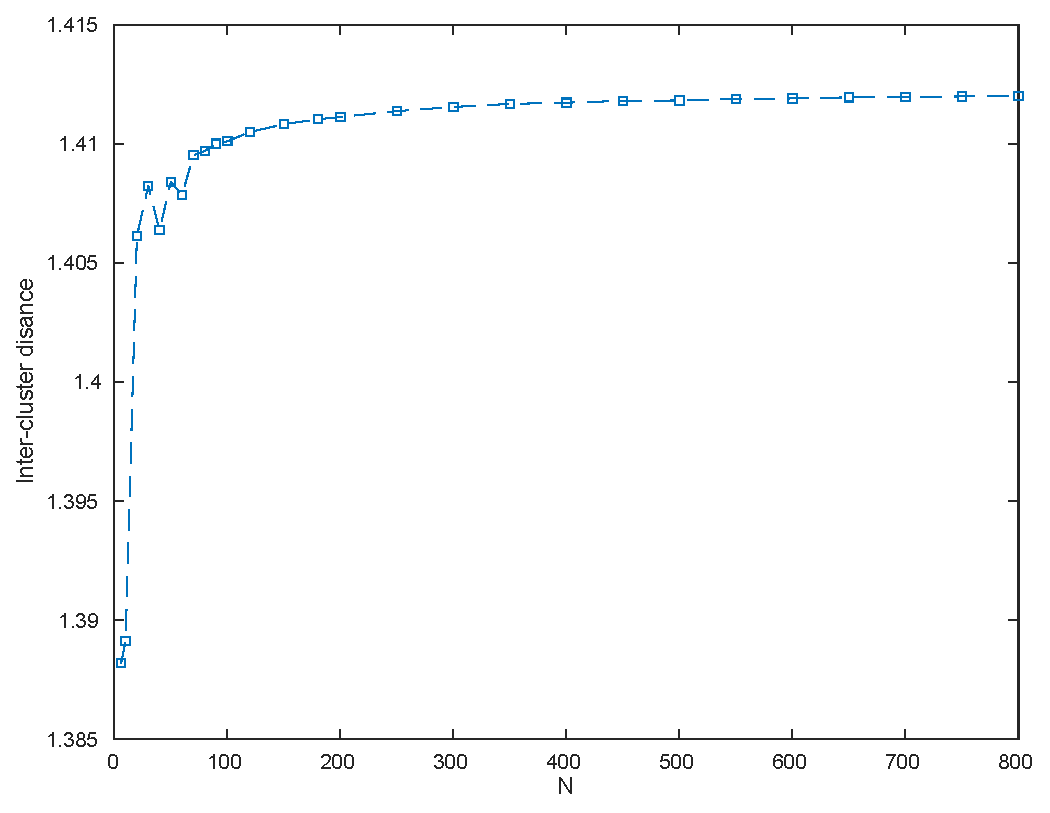
\includegraphics[width = \linewidth]{dvn.eps}
            \caption{Inter-cluster distance for static two cluster state. Simulations were run for various values of \(N\) with \(K = -0.5,J = 0.3,\gamma_1 = 2/3,\gamma_1 = -1/3\). Swarmalators were initially positioned in two equally sized clusters with average phase \(0\) and \(\pi\) and simulations were run for \(T = 300\) time steps.}
            \label{fig:dvn}
        \end{figure}
        \begin{figure}[h!]
            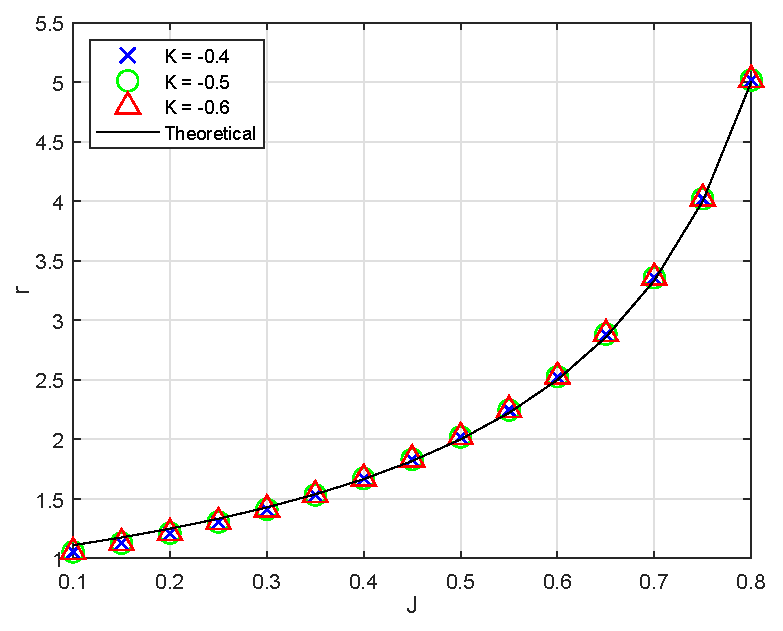
\includegraphics[width = \linewidth]{interClusterNotLog.eps}
            \caption{Inter-cluster distance for varying K. Simulations were run for various values of \(K\) and \(J\) for \(N = 800\). The black line shows the theoretical prediction as per Eq.\ref{eq:eqdist}. The figure justifies that inter-cluster distance is independent of \(K\).}
            \label{fig:KvJ}
        \end{figure}
        Also, from Eq.\ref*{eq:eqdist}, we realize that for \(J > 1\) the two clusters move to infinity. 
    }
    \section{Two clusters with Rogues}
    {
        Two clusters with rouges is a special non-stationary state which occurs for values of \(\gamma_1\) and \(\gamma_2\) ``close'' to \(2/3\) and \(-1/3\) respectively. From our analysis we couldn't conclusively find the exact region where this state was possible. We encountered this state mostly when we ran random simulations with \(\gamma_1 = 2/3\) and \(\gamma_2 = -1/3\). We also tried adding swarmalators in the middle of static two cluster state to understand how \(\gamma_1\) and \(\gamma_2\) influenced the formation of rogues, but we weren't able to get conclusive results. Looking into the dynamics, the presence of rogues caused the clusters to come closer and execute oscillations as the rogues moved back and forth. The system settled down to a stationary state only for the case with one rogue swarmalator. The rogues would always form clusters with similar phase which would pass through each other while moving back and forth. These spacial oscillations causes phase oscillations of the rogues and the clusters. Fig.\ref{fig:PhaseVtimeRogues} shows the phase oscillations of the rogues and clusters. After running the simulation for \(N = 100\) case for \(T = 1000\) time steps, the first half of which were discarded, the phase was averaged for each cluster. The two big cluster had a phase difference of approximately \(\pi\) and the rogues had a phase difference of approximately \(\pi/2\) from the clusters. 

        \begin{figure}[h!]
            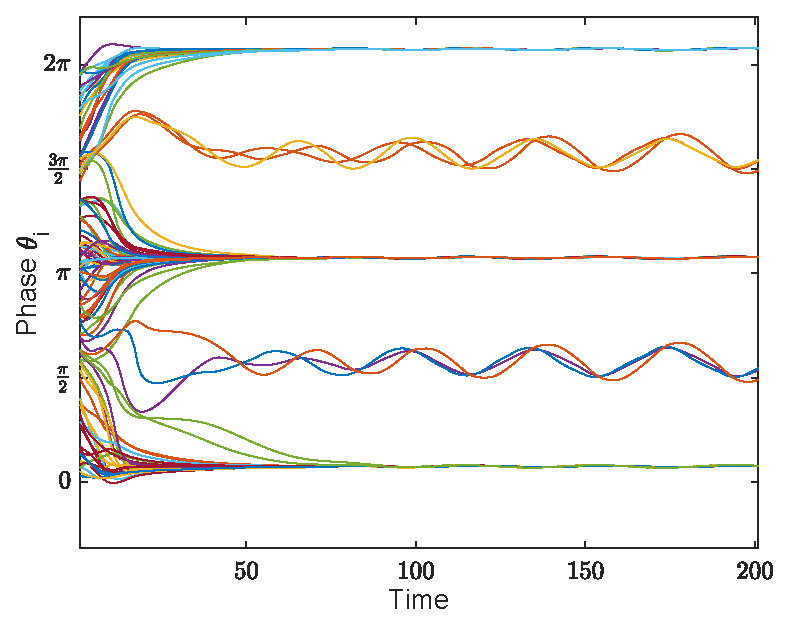
\includegraphics[width = \linewidth]{PhaseVtimeRogues.eps}
            \caption{Phase of Swarmalator Vs Time for two clusters with rogues. The figure shows rogues performing sinusoidal phase oscillations with mean phase \(\pi/2\) off from the big clusters. Simulations were run for \(N = 100\) for 200 time steps with \(\gamma_1 = 2/3\) and \(\gamma_2 = -1/3\).} 
            \label{fig:PhaseVtimeRogues}
        \end{figure}
    }
    \section{Active single cluster state}
    {
        Active single cluster state is a special single cluster state when \(-\gamma_1 < 2\gamma_2\) where \(\gamma_1 < 0\). Due to \(\gamma_1\) being negative, the system prefers to be in a single cluster state, but at the same time, positive \(\gamma_2\) makes the system split into two phase clusters. Such opposite behavior of \(\gamma_1\) and \(\gamma_2\) makes the system reach such a state. Swarmalators along the boundary of phase clusters jump from one cluster to another. Even after running the simulations for a long time \((T > 2000)\), the system didn't show signs of settling down. Fig. \ref{fig:ActiveSingle} shows how the phase is split between the clusters. 
    }
    \section{Active three-four cluster state}
    {
        Active three-four cluster state is a special extension of two cluster with rogues state. Under random runs such a state was never achieved. The state shown in Fig. \ref{fig:Active4Clust} was created by placing 20 swarmalators of phase \(\pi/2\) in the middle of two clusters with phase \(0\) and \(\pi\). The two big clusters are brought together much closer than any other states and there is a smooth gradient of phase within the cluster. The clusters in the center perform random motion within the cluster while the boundary swarmalators of the big clusters perform circular motion. There is no longer back and forth motion of the center clusters. Such a state is also possible with three clusters.
    }
    \section{Static bimodal single cluster state}
    {
        This state is reached when \(J < 0\) with \(K > 0, \gamma_1 < 0\), and \(\gamma_2 > 0\) or \(K < 0, \gamma_1>0\), and \(\gamma_2 < 0\). If sign of \(\gamma_2\) is flipped, the state changes to static async. Here the phase difference between the swarmalators is very close to \(\pi\). A similar state is achieved for \(J = 0\), which is expected since Eq.\ref{eq:space} is phase decoupled. 
    }
    \section{Stability}
    {
        In this section we will briefly look into the stability of the above states. We will focus our analysis into phase stability since stable phase dynamics consequently implies stable spacial dynamics. 
        %Although, the converse does not necessarily hold true. One such case is when there was one swarmalator in the middle. The system showed spacial stability, i.e, it showed no motion after running the simulation for a very long time, but there was one positive eigenvalue in the phase jacobian matrix. Keeping this in mind, we can briefly look into the stability of various states stated before. 
        
        Calculating the jacobian is fairly straightforward for Eq.\ref{eq:phase}. 
        \begin{align}
            \mathbf{J} &= \left(\frac{\partial \theta_i}{\partial \theta_j}\right) \nonumber \\
            &= \frac{K}{N}\begin{cases}
                -\sum_{k \neq i} \frac{\gamma_1 \cos\left(\theta_{k}-\theta_{i}\right) + 2 \gamma_2 \cos \left(2 \left(\theta_k -\theta_i\right)\right) }{\left|\mathbf{x}_{k}-\mathbf{x}_{i}\right|} & i = j  \\
                \frac{\gamma_1 \cos\left(\theta_{j}-\theta_{i}\right) + 2 \gamma_2 \cos \left(2 \left(\theta_j -\theta_i\right)\right) }{\left|\mathbf{x}_{j}-\mathbf{x}_{i}\right|} & i \neq j
            \end{cases}
        \end{align}
        First point of interest in this matrix \(\mathbf{J} \mathbf{1} = \mathbf{0}\). Therefore \(0\) is an eigenvalue. This result was not surprising as we already know that shifting the phase by a constant value does not change the dynamics of the system.  

        For Single cluster case, \(\theta_i = 0\). 
        \begin{align}
            \left.\mathbf{J}\right|_{\theta_i = 0} &= \frac{K}{N}\begin{cases}
                -\sum_{k} A_{ik} (\gamma_1 + 2\gamma_2) & i = j  \nonumber \\
                A_{ij}(\gamma_1 + 2\gamma_2) & i \neq j
            \end{cases}\\
            &= -\frac{K}{N}(\gamma_1 + 2\gamma_2) \begin{cases}
                \sum_{k} A_{ik} & i = j \nonumber\\
                -A_{ij} & i \neq j
            \end{cases}\\
            &= -\frac{K}{N}(\gamma_1 + 2\gamma_2) \mathbf{M}
        \end{align}
        where \(A_{ij} = |\mathbf{x}_j - \mathbf{x}_i|^{-1}\) with \(A_{ii} = 0\). Here \(\mathbf{M}\) is a weighted Laplacian matrix and therefore semi-positive definite. Therefore the eigenvalues of \(J\) are 
        \begin{align}
            \mathbf{J} : \begin{cases}
                \lambda_i \geq 0 & \text{if } -K(\gamma_1 + 2\gamma_2) > 0 \\
                \lambda_i = 0 & \text{if } -K(\gamma_1 + 2\gamma_2) = 0 \\
                \lambda_i \leq 0 & \text{if } -K(\gamma_1 + 2\gamma_2) < 0 
            \end{cases}
        \end{align} 
        This result gives us deep insight about single cluster stability. For a fixed value of \(K < 0\), single cluster state is only stable when \(\gamma_1 + 2\gamma_2 < 0\). For any other values of \(\gamma_1,\gamma_2\), the system will eventually break into two clusters. Stability of single cluster for all the three cases is shown in Fig.\ref{fig:case1},\ref{fig:case2},\ref{fig:case3}.
        \begin{figure}[h!]
            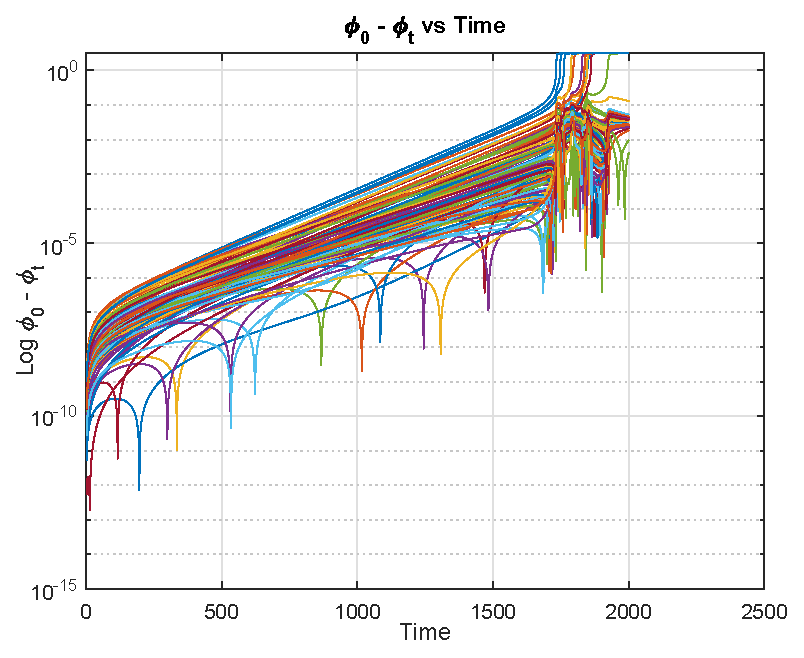
\includegraphics[width = \linewidth]{unstablePositive.eps}
            \caption{Unstable single cluster case 1. In this case \(\gamma_1 + 2\gamma_2 = 0.005 > 0\). From the figure, we can see that small phase perturbation of order \(10^{-8}\) grow exponentially until the system breaks into two clusters.}
            \label{fig:case1}
        \end{figure}
        \begin{figure}[h!]
            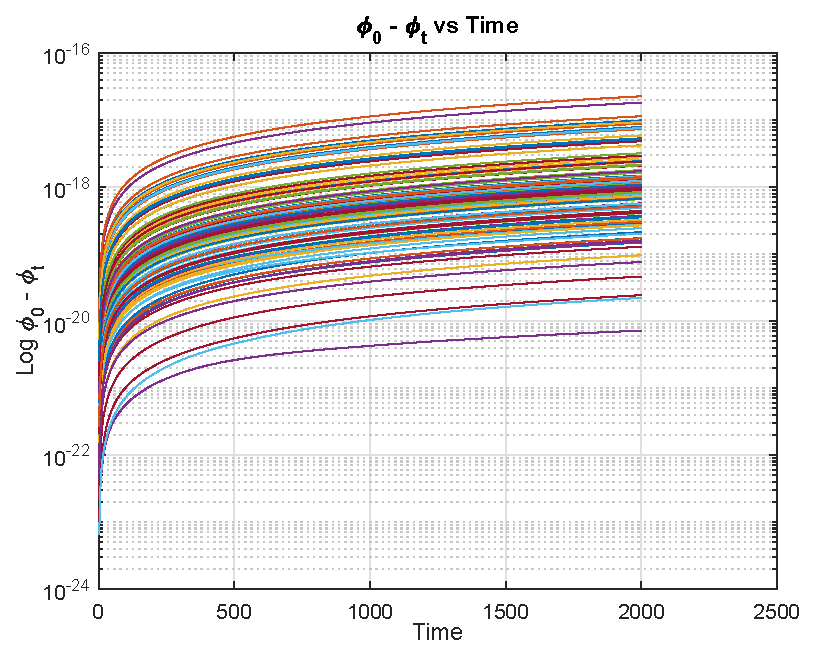
\includegraphics[width = \linewidth]{LinearUnstable.eps}
            \caption{Unstable single cluster case 2. In this case \(\gamma_1 + 2\gamma_2 = 0\). Here small phase perturbation of order \(10^{-8}\) grow linearly. Due to linear growth, it will take a significantly large amount of time for the system to break into two clusters.}
            \label{fig:case2}
        \end{figure}
        \begin{figure}[h!]
            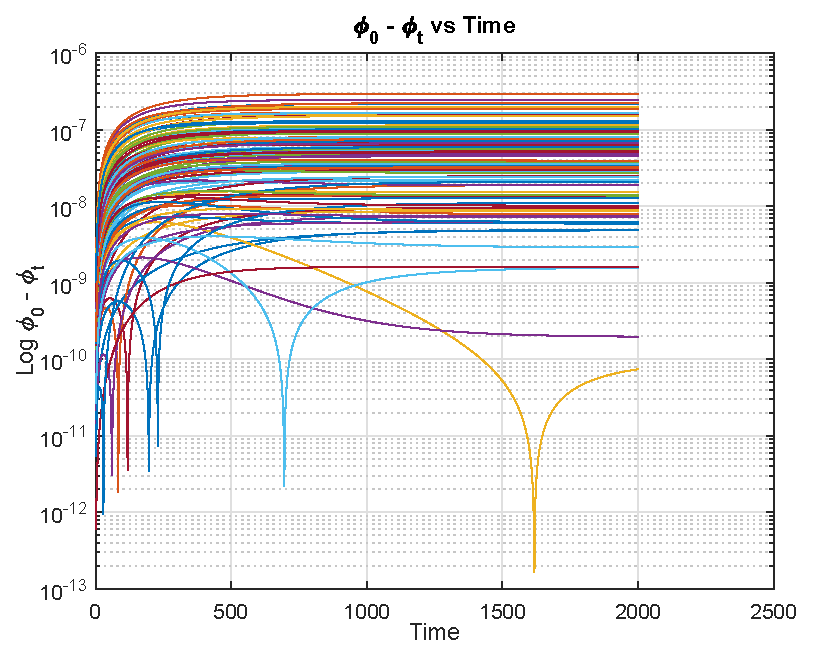
\includegraphics[width = \linewidth]{negativeStable.eps}
            \caption{Stable single cluster case 3. Here small phase perturbation of order \(10^{-8}\) show no growth after 1700 time steps. This shows that the system has attained a new equilibrium.}
            \label{fig:case3}
        \end{figure}

        For two cluster case, we couldn't arrive at a similar analytical solution like the single cluster case. Nevertheless, we numerically calculated the eigenvalues of phase jacobian matrix to understand the stability of this state. We constructed two clusters with phase \(0\) and \(\pi\) respectively, and ran the simulation for \(\gamma_1 = 2/3\), \(\gamma_2 = -1/3\) for \(T = 2000\) time steps for the system to reach equilibrium. Then we added perturbed phase by adding small random numbers of order \(10^{-8}\). We changed the values of \(\gamma_1\),\(\gamma_2\), ran the simulation for \(T = 2000\) time steps and calculated the phase jacobian matrix at end time step. We found that for \(\gamma_1 + 2\gamma_2 \leq 0\), the system was unconditionally stable, i.e, all eigenvalues of phase jacobian matrix was \(\leq 0\). When \(\gamma_1 + 2\gamma_2 \geq 0.09\), the phase jacobian matrix had positive eigenvalues and the system eventually destabilized into active phase wave. 

        For static bimodal single cluster state, the phase jacobian matrix had negative eigenvalues, implying the state is in-fact static and stable. Adding small perturbation to this state always stabilized to a new equilibrium.  

        Finally, we looked into the eigenvalues of active states, and as expected, they had positive eigenvalues.
    }
}

\section{Periodic motion of Rogues}
{
    In this section, we will briefly look into periodic motion of rogues in two cluster with 3-3 rogues as shown in Fig. \ref{fig:twoClustersWithRogues}. Due to the static nature of the two big clusters and a small number of rogues, we expected the rogues to show periodic cyclic motion. To test this argument, we ran the simulation for 4000 time steps, the first half of which was discarded, and plotted the motion of the rogues to check if they formed closed loops. They did form closed loops as shown in Fig. \ref{fig:cyclicMotion}, but there weren't completely symmetric. Such closed loops were not found when there were large number of rogues. This suggest that there is a threshold over which chaos is observed in the dynamics of rogues. 
    
    \begin{figure}
        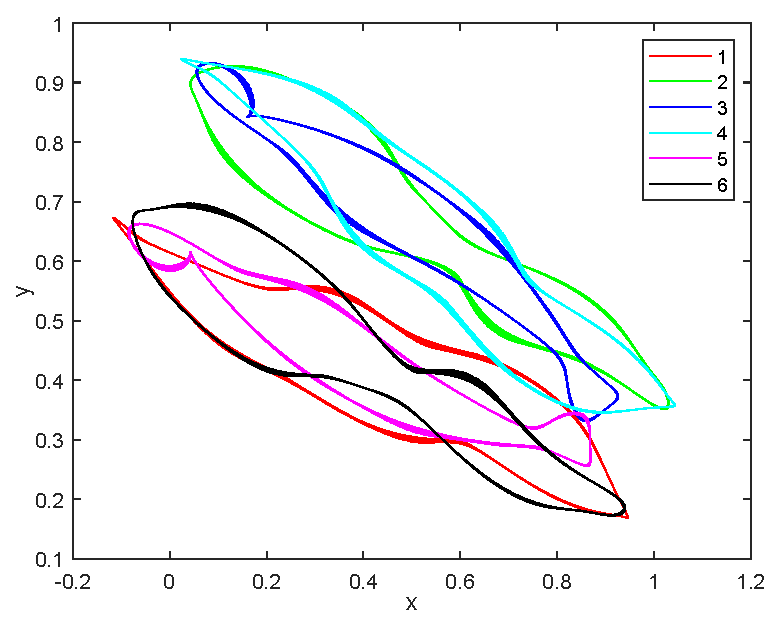
\includegraphics[width = \linewidth]{cyclicMotion.eps}
        \caption{Periodic motion of 3-3 rogues in two clusters with rogues state. Here particle 1,2,and 3 form one rogue cluster and the rest form another rogue cluster.}
        \label{fig:cyclicMotion}
    \end{figure}
}
\section{Circular ring state}
{
    In a search for more stable states, we encountered a special unstable equilibrium state which could be achieved by careful arrangement of swarmalators. It is achieved by placing swarmalators around a circle of half unit radius with a single swarmalator in the center. The circumferential and central swarmalators have a phase difference of \(\pi\). The arrangement of swarmalators is shown in Fig. \ref{fig:circleArr}. Initially, the system collapses to a stable radius and maintains approximately the same radius for some time. After a critical time, the system destabilizes into two clusters. This result is shown in Fig. \ref{fig:radVtime}. We also looked at the distance between the centroid of the circumferential swarmalators and the center swarmalator. From Fig. \ref{fig:centerDistVtime}, we realized that a small perturbation in the arrangement of swarmalators grows exponentially until the system destabilizes into two clusters. To check if this destabilization was due to the numerical solver, we changed the absolute and relative error tolerance to \(10^{-10}\) and this resulted in a slight increase in stable time. Further decrease in error order did not increase the stable time of the system. We also ran the simulation in single precision mode by adding an error term of order \(10^{-8}\) to the solver function. This change to single precision decreased the stable time by half as shown in Fig.\ref{fig:centerDistVtimeError}. These tests does not confirm the numerical instability of the ode solver, but it does give insight into the sensitivity of such configuration. 
    \begin{figure}
        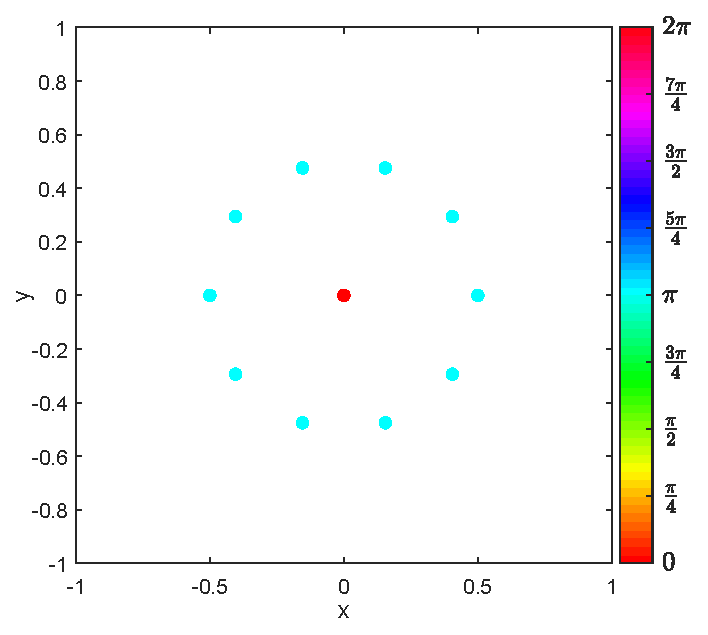
\includegraphics[width = \linewidth]{circleArrangment.eps}
        \caption{Circular arrangement of swarmalators. Here the central swarmalator has phase \(0\) and the circumferential swarmalators have a phase \(\pi\). The system has \(N = 11\) swarmalators with \(\gamma_1 = 2/3,\gamma_1 = -1/3\)}
        \label{fig:circleArr}
    \end{figure}
    \begin{figure}
        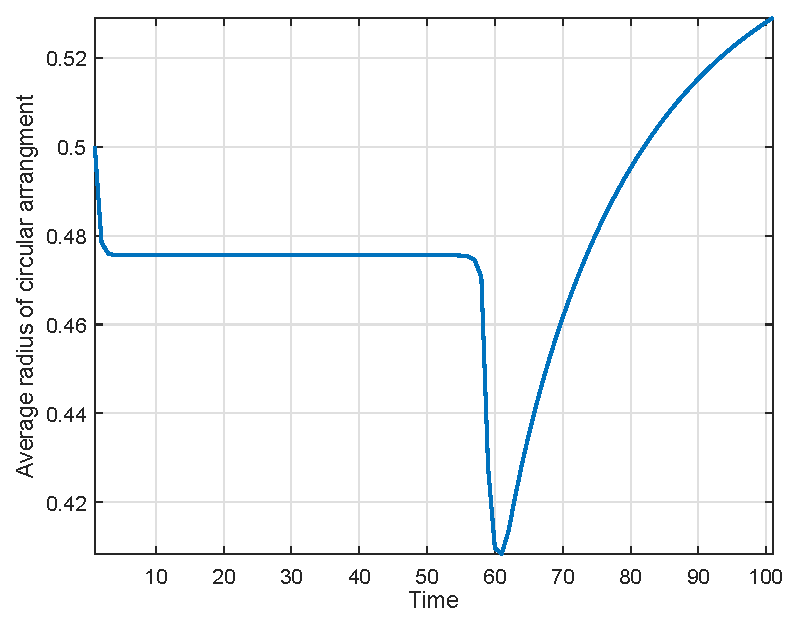
\includegraphics[width=\linewidth]{radiiVtime.eps}
        \caption{Average distance of the swarmalators from the center. The circumferential swarmalators collapse to a stable radius and after a while it destabilizes into two clusters.}
        \label{fig:radVtime}
    \end{figure}
    \begin{figure}
        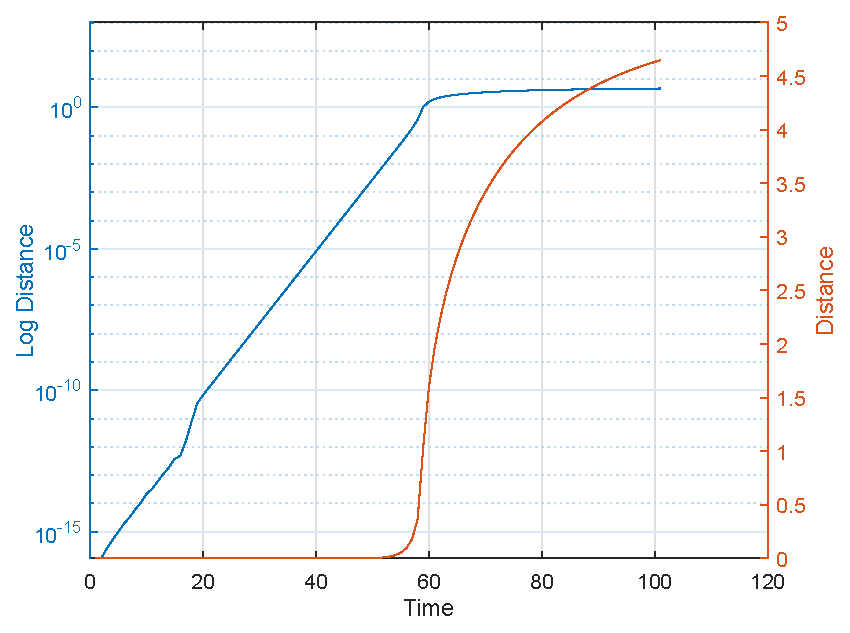
\includegraphics[width = \linewidth]{centerDistVtime.eps}
        \caption{Distance between the centroid of circumferential swarmalators and center swarmalator. We can see that a small perturbation of order \(10^{-16}\) builds up exponentially until the system destabilizes into two clusters}
        \label{fig:centerDistVtime}
    \end{figure}
    \begin{figure}
        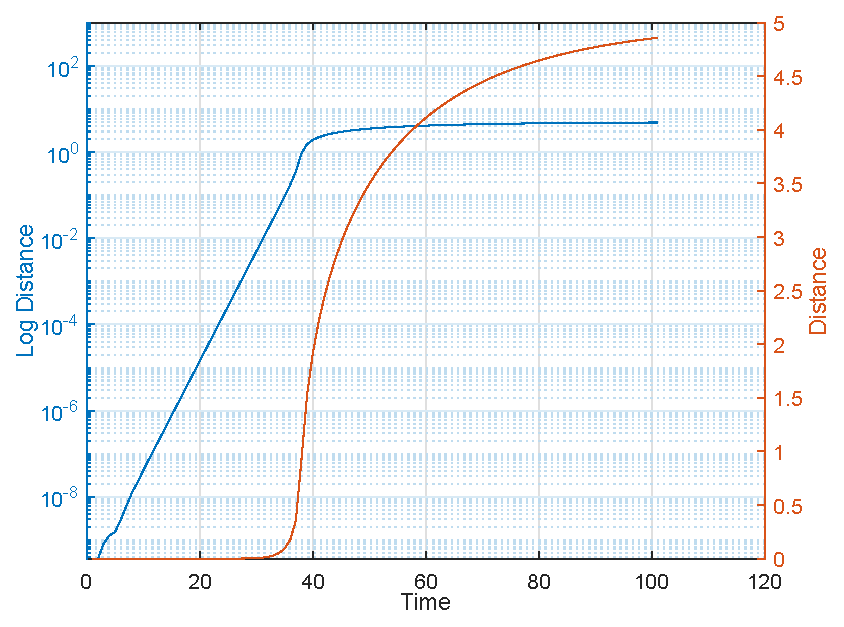
\includegraphics[width = \linewidth]{centerDistVtimeError.eps}
        \caption{Distance between the centroid of circumferential swarmalators and center swarmalator run at single precision mode. Single precision mode was simulated by adding random numbers of order \(10^{-8}\) to the solver function. Comparing with Fig.\ref*{fig:centerDistVtime}, the stable time has been almost reduced by half.}
        \label{fig:centerDistVtimeError}
    \end{figure}
}

\section{Phase Variation within the clusters}
{
    So far, we have explored the collective behaviour of swarmalator in forming clusters. In this section, we will briefly talk about the behaviour of swarmalators within the cluster formation. For static two cluster case, there was little to no phase variation within the cluster. The calculated standard deviation of phase within the cluster was \(2.678 \times 10^{-17}\), which for all numerical purpose is effectively zero. This is indeed quite surprising as we expected a phase gradient within the cluster due to the presence of the other cluster. Finally, adding random phase variations within the cluster led the cluster to stabilize to a different constant uniform value throughout the cluster. The average phase difference between the cluster was still approximately \(\pi\). 

    Static bimodal single cluster is a special case where \(J = 0\). The single cluster behaviour was expected as the system is effectively phase decoupled, i.e, Eq.\ref{eq:space} has no phase term. This results in a single cluster lattice structure where the phase stabilizes to either \(0\) or \(\pi\). Fig.\ref{fig:staticSingleClusterState} shows the structure after the system settles.

    Finally, we looked into two cluster state with rogues. To amplify the phase variations within the cluster, we ran the simulations for \(N = 400\). After the system settled into two clusters with rogues in the middle, the clusters show oscillatory phase distribution within the cluster, as shown in Fig.\ref{fig:phaseVar}. There was a smooth gradient in phase, and the two clusters showed opposite phase distribution as the rogues moved back and forth. %As we stated before, the two clusters were much closer due to the presence of rogues

    \begin{figure}[h!]
        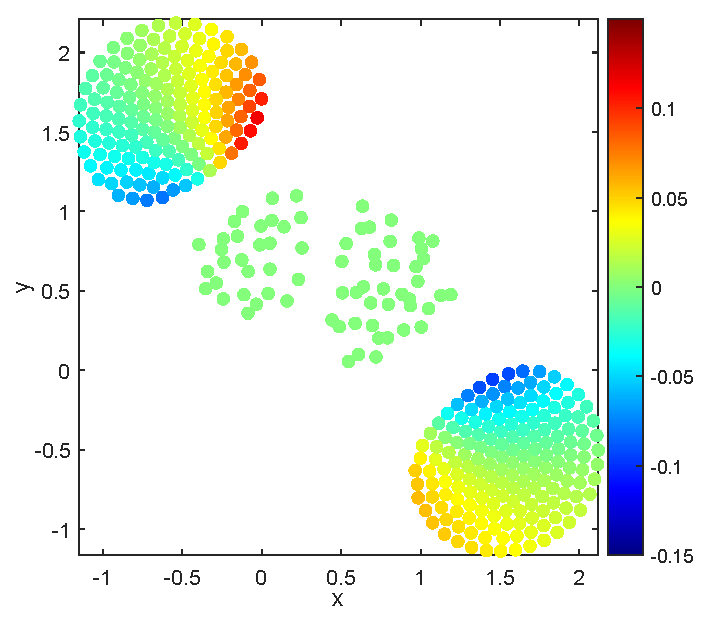
\includegraphics[width = \linewidth]{phaseVar.eps}
        \caption{Phase variation within the cluster. This simulation was run for \(N = 400\) with \(\gamma_1 = 2/3,\gamma_1 = -1/3\). The phase of each cluster was centered to zero by using the average phase of the cluster. The color gradient shows the variation of phase within the cluster. The phase of all rouges (center swarmalators) was set to zero for better visualization. }
        \label{fig:phaseVar}
    \end{figure}
}
\noindent

%\section{Simplified model}

\section{Front end application}
{
    \begin{figure}[h!]
        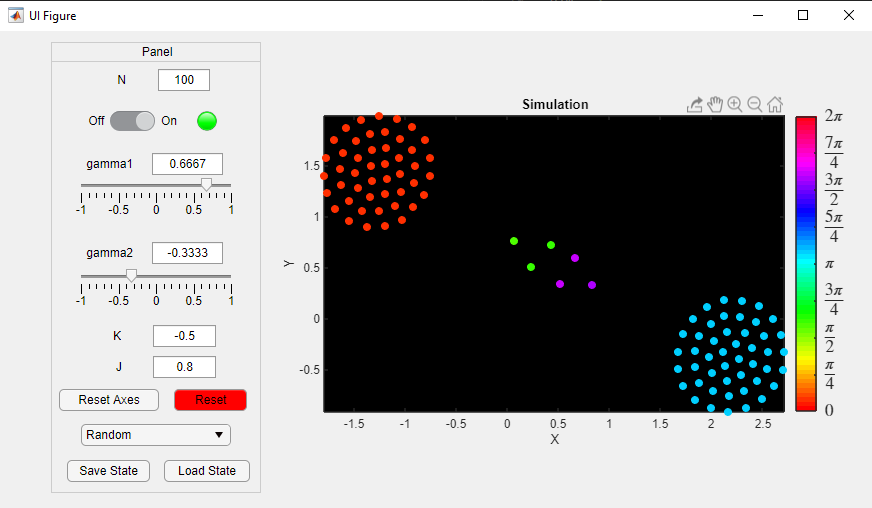
\includegraphics[width = \linewidth]{gui.png}
        \caption{GUI interface.}
    \end{figure} 
    To showcase the dynamics of the model in a user friendly manner, we made a GUI which displays the simulation while the model is being solved in the background. MATLAB App Designer was used to make the GUI because of its ease of use and user friendly interface. We implemented callback functions which would dynamically change model parameters and these changes can be almost seen instantaneously. We made our own ODE-plotter function which would plot output as it is being calculated by ode45. It would terminate when any of the callback functions are executed, change the model parameters, and continue integration. For reasons which are unknown, implementing the model in GUI slowed down integration considerably. Even then, the animation was fast enough to show how the system responded for different parameters. 
}
\section{Discussion}
{
    We have investigated the collective dynamics of the extended swarmalator model. These are mobile particles which have both phase and spatial degrees freedom. Furthermore, their phase and spatial dynamics are coupled. In the original single phase model, there were rich spatiotemporal patters, but they were constrained to a single cluster unit. The extended model not only showed all the states in the single phase model, but showed a variety of new states. We performed some basic analysis on these states numerically and analytically. As \(\gamma_1, \gamma_2\) could represent the fourier coefficient of some general function, this analysis could help us predict the stable states of such a system. There is a very good possibility that there are many more states, as we haven't comprehensively explored the space defined by the parameters \((K,J,\gamma_1,\gamma_2)\) given its large in size. These new states could provide us with deep insight about the our model, and maybe help formulate a model which would show a new landscape of emergent behavior. One possible area of future research would be to use collective coordinates to reduce high dimensional Swarmalator system, to a few number of active degrees of freedom. This could simplify the dynamics and provide insight about the behavior of rogue swarmalators. One possible real-world swarmalators are biological micro-swimmers, such as spermatoza, which exhibit rich swarming behavior. The phase variable in such sperms could be the rhythmic beating of the sperm's tail.which can synchronize with other sperms. One route to increase more realism would be to study complex coupling parameters as functions of position or phase, or choosing more complicated interaction functions \(\mathbf{I}_{att},\mathbf{I}_{rep},G,H_{att}\).

    All data files used to create plots, run simulations, and GUI will be available at github repository ``ankithadas/Extended-Swarmalator-Model''. 
}

%\section{References}
% CHALMERS UNIVERSITY OF TECHNOLOGY (2019). Methodology for Topology and Shape Optimization: Application to a Rear Lower Control Arm. [online] Sweden. Available at: \url{https://www.chalmers.se/SiteCollectionDocuments/Produkt-%20och%20produktionsutveckling/Nationell%20kompetensarena%20kring%20produktoptimering/Methodology_for_Topology_and_Shape_Optimization_report.pdf [Accessed 5 Nov. 2019].}
\bibliography{refs}
\bibliographystyle{IEEEtran}
\end{document}